\documentclass[adobefonts, nocap]{ctexart}
\usepackage{amsmath}
\usepackage{amsfonts}
\usepackage{listings}
\usepackage{xcolor}
\usepackage{graphicx}
\usepackage{siunitx}
\usepackage{hyperref}
\hypersetup{
  colorlinks = true,
  linkcolor = blue,
  unicode = true
}
\lstset{
  language = C,
  basicstyle = \small\ttfamily,
  keywordstyle = \small\ttfamily\color{red},
  stringstyle = \color{gray},
  numbers = left,
  numberstyle = \tiny,
  numbersep = 5pt,
  frame = leftline,
  showstringspaces = false
}
\begin{document}
  \title{计算机系统结构第二次实验}
  \author{李雨田\hspace{1em}2010012193\hspace{1em}计14}
  \maketitle
  \tableofcontents
  \section{设计思路}
    在设计的时候主要参考了Scott McFarling的Combining Branch Predictors和一些其他的文档.根据调研的文档,基本上单一预测机制中gshare已经是达到最好的效果了.具体的测量结果参见下图.可见在$32$KB的存储空间下gshare的确是性能最优的.

    \begin{center}
      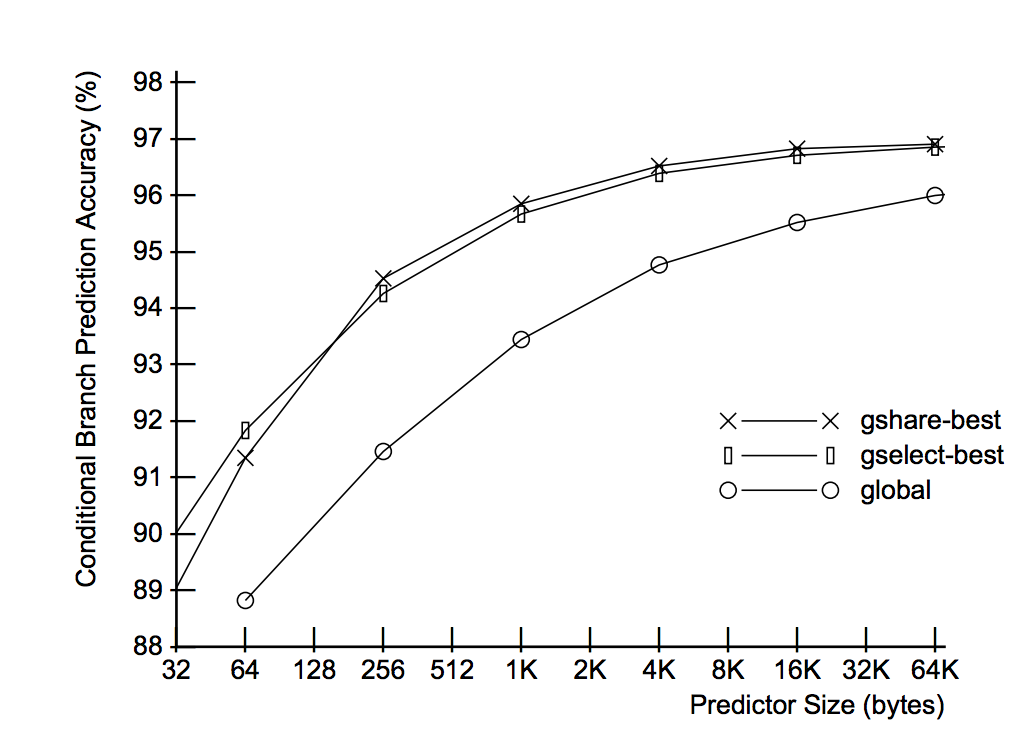
\includegraphics[width=22em]{1.png}
    \end{center}

    如果要达到更好的效果,则要使用复合的分支预测机制.对于几种常用的复合的方法,同样有测量结果,参见下图.在$32$KB的存储空间下,
    local和gshare的复合的性能是最好的.

    \begin{center}
      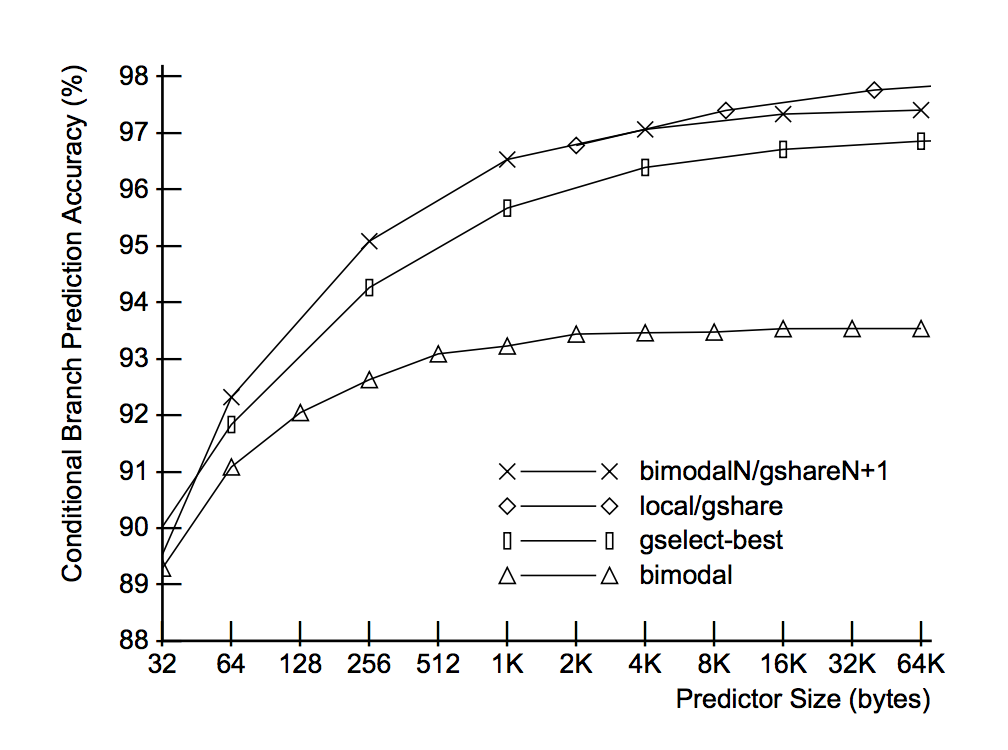
\includegraphics[width=22em]{2.png}
    \end{center}

    为此首先需要一对local表.第一个表有$2^{14}$项,每一项有$13$bit,使用PC值的低$14$位索引,记录当前对应分支的历史执行情况.然后根据当前
    分支历史执行情况,在第二个表中索引.第二个表显然需要有$2^{13}$项,每一项有$2$bit,为饱和计数器.

    注意到虽然在第一个表中会根据PC值索引到对应分支的历史执行情况,但是可能出现多个分支对应于同一项的问题.

    然后gshare表有$2^{13}$项,每一项有$2$bit,为饱和计数器.使用PC值和全局历史执行情况的异或之后的低$13$位进行索引.

    最后还需要一个meta表,有$2^{13}$项,每一项有$2$bit,为饱和计数器.同样使用PC值和全局历史执行情况的异或之后的低$13$位进行索引.此表记录的是采用gshare表的预测还是local表的预测.

    初始情况下所有饱和计数器为$2$,即weakly taken. meta表表项默认为$1$, 即weakly prefer local.

    在运行的时候根据实际分支情况修改相应的表项.需要修改对应的local表和gshare表的饱和计数器.并且当一种预测机制正确而另一种错误的时候,
    要在meta表中修改饱和计数器,使其偏向于正确的预测机制.
  \section{存储空间}
    local表大小为$2^{14}\times 13+2^{13}\times 2=229376$bit.

    glocal表大小为$2^{13}\times 2=2^{14}$bit.

    meta表大小同样为$2^{14}$bit.

    加起来总和为$2^{18}$bit,即$32$KB.

    最后还有$13$bit的全局历史执行情况.
  \section{实验结果}
    在测试数据上达到了平均$4.605$的MPKI.对比同样使用$32$KB存储空间的gshare,其MPKI为$5.196$,相比降低了$11.4\%$.在每一个测试点上进行对比可以发现,并不是所有的测试点都比gshare好.大部分时候不相上下,或者有少量的减小.但是在某些测试点,比如
    LONG-SPEC2K6-06上,优化效果明显,使得最后整体成绩偏好.
\end{document}
